% ============================================================================
% advisor_memo.tex
% Intuitive 5-page overview of the MTU15 thesis project for the advisor.
% Companion: descriptive_facts.tex (detailed working notes).
%
% SKELETON ONLY. Section structure, figure placeholders, and table skeletons.
% Prose to be written by the author.
% ============================================================================

\documentclass[11pt]{article}

\usepackage[margin=1.9cm]{geometry}
\usepackage{graphicx}
\usepackage{amsmath, amssymb}
\usepackage{booktabs}
\usepackage{array}
\usepackage[table]{xcolor}
\usepackage{hyperref}
\hypersetup{colorlinks=true, linkcolor=blue!50!black, urlcolor=blue!50!black}
\usepackage{microtype}
\usepackage{enumitem}
\setlist[itemize]{leftmargin=*, itemsep=2pt, topsep=2pt}
\usepackage{titlesec}
\titlespacing*{\section}{0pt}{8pt}{4pt}
\titlespacing*{\paragraph}{0pt}{4pt}{6pt}
\renewcommand{\arraystretch}{1.05}

\graphicspath{{../../figures/thesis/}{../../figures/working/}}

\title{\vspace{-1.5cm}\large MTU15 thesis project --- intuitive overview\vspace{-0.4cm}}
\author{\normalsize Pablo Paramio Mart\'in}
\date{\normalsize\today}

\begin{document}
\maketitle
\vspace{-0.8cm}

% =====================================================================
% PAGE 1: The question
% =====================================================================
\section*{1. The question}

\paragraph{Market structure (reform calendar in one paragraph).}
% TODO: Spanish wholesale; auction layers (DA, IDA auctions, continuous, balancing);
%       three reforms (IDA-sessions 2024-06, ISP15 2024-12, MTU15-IDA 2025-03, MTU15-DA 2025-10);
%       what each reform changed in market design and in settlement.

\paragraph{Who actually sets the price (NOT a priori CCGT).}
% TODO: tech-level price-setter shares (see descriptive_facts §X for the table);
%       hydro dominates, CCGT is ~9% — but CCGT is the focal technology because
%       of strategic profile, not because it's most often marginal.

\paragraph{Why this matters.}
% TODO: granular pricing as a NEW STRATEGIC MARGIN that didn't exist before;
%       framing in terms of within-hour discrimination opportunity for whichever
%       units are at or near the margin in critical hours.

\paragraph{Outcomes we care about, and why.}
\begin{itemize}
\item % TODO: bid-shape divergence
\item % TODO: quarter-level cleared quantities (q1, q2)
\item % TODO: within-hour clearing-price dispersion
\item % TODO: mark-up / market-power proxies
\end{itemize}

% =====================================================================
% PAGE 2: Variation across hours
% =====================================================================
\section*{2. Variation across hours: where granularity has economic content}

\paragraph{Intuition.}
% TODO: short paragraph on within-hour residual-demand variation as the
%       structural condition for granularity to matter.

\paragraph{Classifier.}
% TODO: sigma_within(h,d) definition; data window 2023-01-01 to 2026-05-14
%       (ENTSO-E 15-min ISP, A65 load + A75 wind+solar actuals).

\paragraph{What we see.}
\begin{itemize}
\item % TODO: critical hours 5--9, 16--22, sigma in [522, 1303] MW
\item % TODO: flat hours 1--3, sigma in [336, 357] MW
\item % TODO: midday hours 11--14, sigma in [468, 502] MW, excluded (solar-marginal regime)
\end{itemize}

\paragraph{Validation.}
% TODO: post-MTU15-DA within-hour DA quarter-price std: 6.6 EUR/MWh critical vs
%       2.1 flat (3x). Same falsifier on CCGT price-setting share (9.1% crit vs 9.0% flat).

\begin{figure}[h]
\centering
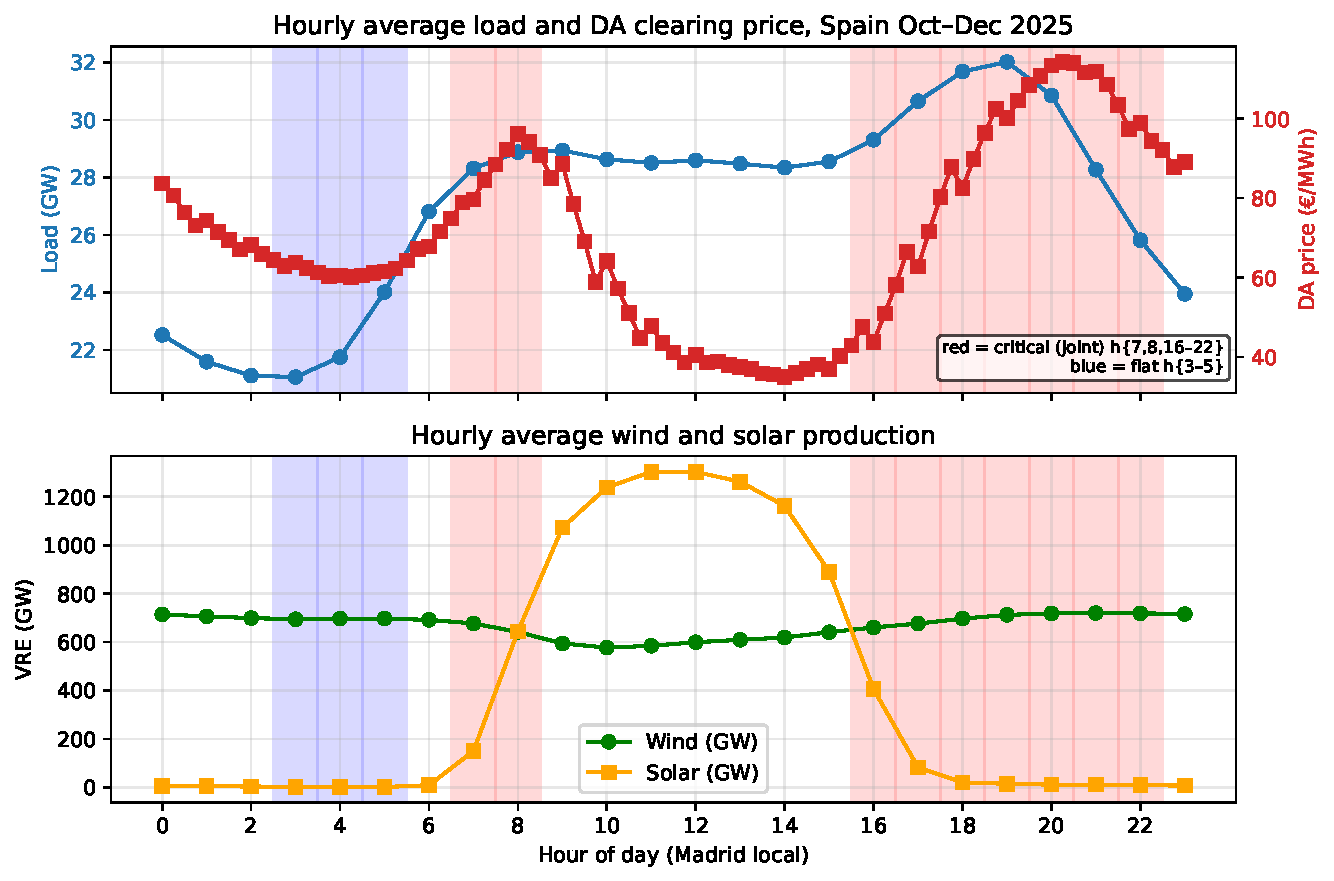
\includegraphics[width=0.72\textwidth]{fig_critical_hours_calibration.pdf}
\caption{\small % TODO: caption.
}
\label{fig:sigma_within}
\end{figure}

% =====================================================================
% PAGE 3: Variation across firms / technologies
% =====================================================================
\section*{3. Variation across firms and technologies: how do CCGTs bid?}

\paragraph{The object.}
% TODO: 4 quarter supply curves per unit per hour; need to measure how much
%       they differ in the band that matters for clearing.

\paragraph{Metric: $D_w$.}
% TODO: kernel-weighted area between curves in the band $\pm 50$ EUR/MWh around
%       the hour-mean clearing price; aggregate the 6 within-hour pairs by max.

\paragraph{Decomposition: $\Delta p$ vs $\Delta q$.}
% TODO: upper bound D_w <= Delta_p * M_i + 2h * Delta_q; what each channel
%       means in plain terms.

\paragraph{What we see (post-MTU15-DA, critical hours, CCGT, Oct--Dec 2025).}
\begin{itemize}
\item % TODO: GN dominates $\Delta q$
\item % TODO: GE leans on $\Delta p$
\item % TODO: IB and HC negligible on both
\item % TODO: flat hours $\approx 0$ across firms
\end{itemize}

\begin{figure}[h]
\centering
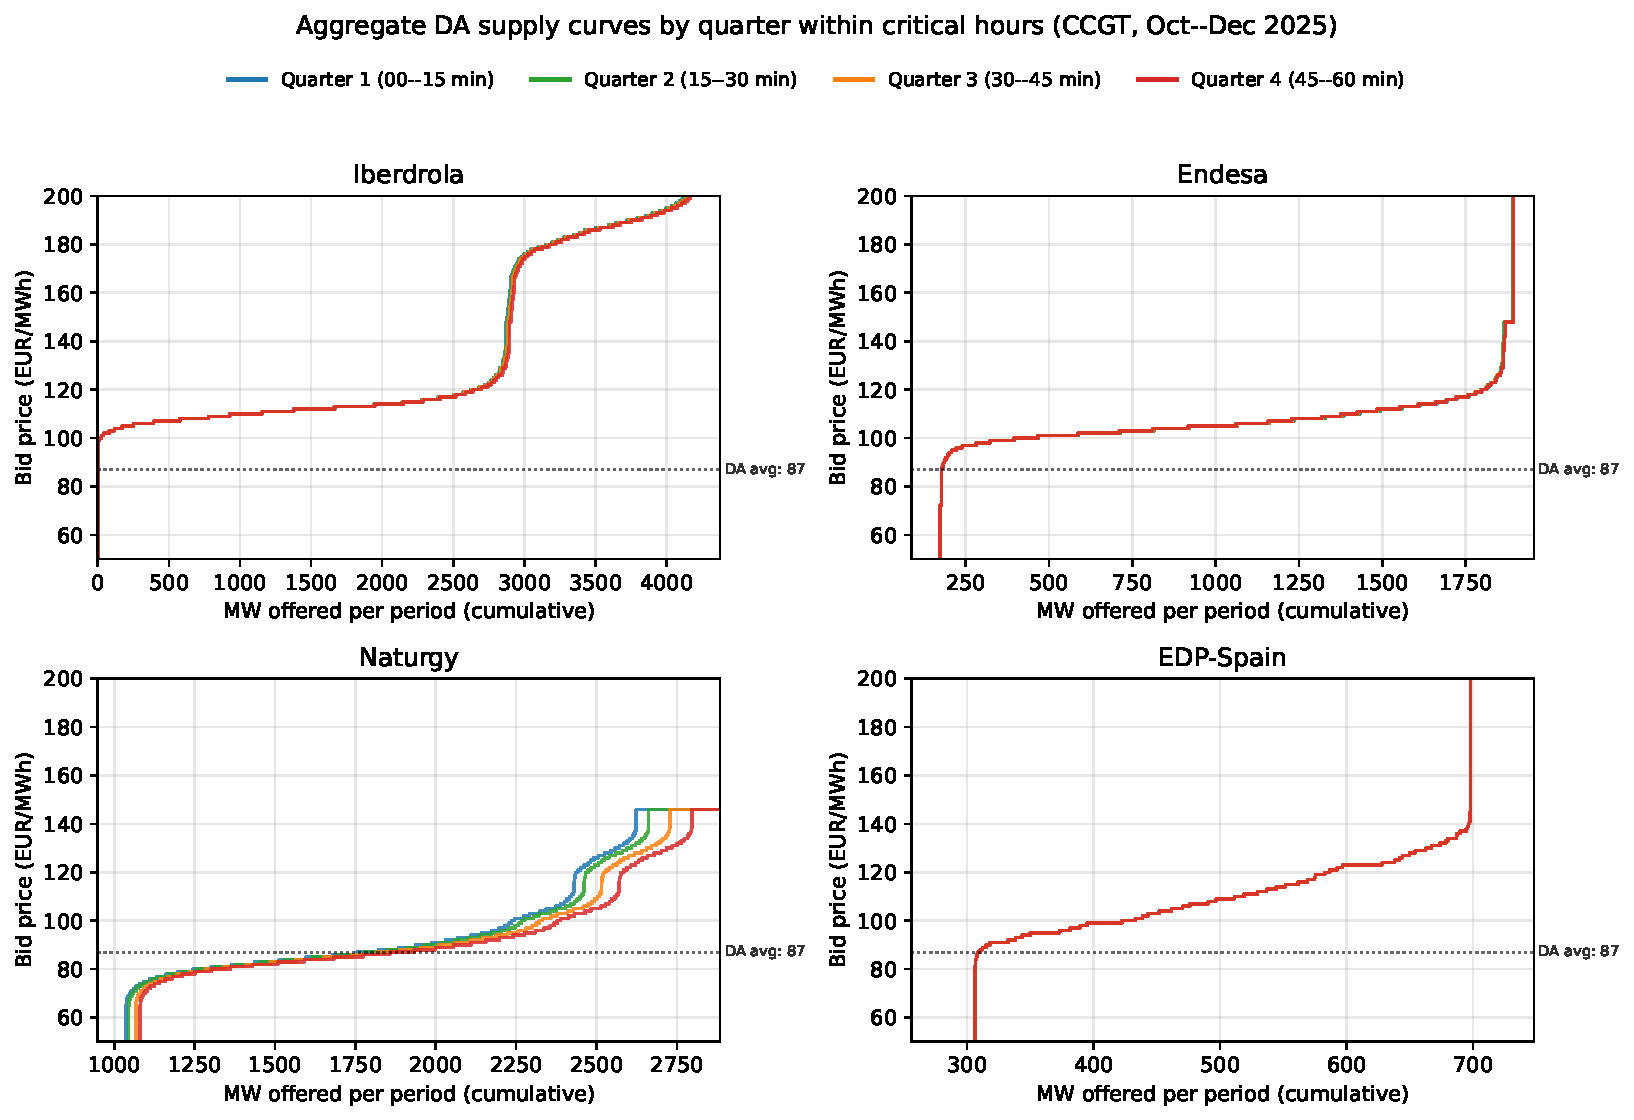
\includegraphics[width=0.92\textwidth]{fig_per_firm_bid_curves_quarters_ccgt.pdf}
\caption{\small % TODO: caption.
}
\label{fig:perfirm}
\end{figure}

\paragraph{Operational vs strategic decomposition.}
% TODO: how we separate physical-constraint shape variation from strategic
%       variation (price-setter restriction).

% =====================================================================
% PAGE 4: Confounders: blackout + reforzada
% =====================================================================
\section*{4. The 2025 regulatory shock: blackout and reinforced operation}

\paragraph{The blackout (28 April 2025).}
% TODO: pan-Iberian blackout; XBID suspension; entrance into reforzada posture.

\paragraph{What ``reforzada'' does in practice.}
\begin{itemize}
\item % TODO: PO-3.x forced CCGT inclusion (+1,044 GWh/mo post-blackout)
\item % TODO: PO-7.4 zonal reactive market (June 2025)
\item % TODO: CNMC enforcement (April 2026 cohort, ~100 expedientes)
\end{itemize}

\paragraph{What this lets us claim.}
% TODO: within a tight window around each reform date, regulatory state is
%       approximately constant; sharp changes at the reform date are
%       attributable to the reform itself, not to the broader 2025 turmoil.

% =====================================================================
% PAGE 5: Reform windows + outcomes
% =====================================================================
\section*{5. Reform windows we use, and outcomes we measure in each}

\paragraph{Strategy in one sentence.}
% TODO: tight window per reform; reforzada (and other regulatory confounders)
%       are constant within window; reform variation stands out.

\paragraph{The reform calendar and our windows.}

\begin{center}
\footnotesize
\begin{tabular}{p{2.6cm} p{3.2cm} p{8.8cm}}
\toprule
\textbf{Reform} & \textbf{Date} & \textbf{Window and why} \\
\midrule
% TODO: IDA: 6 MIBEL --> 3 European sessions & 2024-06-14 & ...
\\ \addlinespace
% TODO: ISP15 & 2024-12-01 & (quantities at 15-min, prices still hourly --- the
%       genuinely new ex-ante information environment vs the prior regime) & ...
\\ \addlinespace
% TODO: MTU15-IDA & 2025-03-19 & ...
\\ \addlinespace
% TODO: MTU15-DA & 2025-10-01 & ...
\\
\bottomrule
\end{tabular}
\end{center}

\paragraph{Outcomes we measure in each window.}

\begin{center}
\footnotesize
\begin{tabular}{p{4.4cm} p{12.0cm}}
\toprule
\textbf{Outcome} & \textbf{What it tells us / why it matters} \\
\midrule
% TODO: D_w bid-shape divergence
\\ \addlinespace
% TODO: Delta_p / Delta_q channel shares
\\ \addlinespace
% TODO: quarter-level CCGT cleared output (q1, q2)
\\ \addlinespace
% TODO: mark-up proxies
\\ \addlinespace
% TODO: price-setter frequency by firm and hour-class
\\
\bottomrule
\end{tabular}
\end{center}

% =====================================================================
% PAGE 6+: MTU15 effect --- critical/flat identification (ID15 and DA15)
% =====================================================================
\section*{6. MTU15 effect: critical/flat identification (ID15 and DA15)}

\paragraph{Strategy.}
\textit{(Gap to write: 3--4 sentences recapping the critical/flat identification --- critical hours $\{5,6,7,8,16,\dots,22\}$ are where within-hour residual demand varies and MTU15 has economic content; flat hours $\{1,2,3\}$ are the within-day control where MTU15 should not matter; the (critical $-$ flat) differential across the reform date isolates the MTU15 effect from any day-level shock that hits both classes proportionally.)}

\subsection*{6.1 Specifications}

Let $u$ index a unit, $d$ a date, $p$ a market period (hour pre-MTU15, quarter post), $h$ the clock-hour, $s$ the IDA session, $T_r$ the reform date, $\mathcal{C}$ the critical-hour set. All sell-side, in-band $|p_{\text{bid}} - \text{MCP}| \le 140$ EUR/MWh.

\textbf{Spec A --- per-curve functional outcomes} $Y \in \{\sigma_p, N_{\text{eff}}\}$, panel $(u,d,p[,s])$:
\[
Y_{u,d,p[,s]} \;=\; \alpha + \alpha_u + \delta_d + \gamma_h + \beta\,\mathbf{1}\{d \ge T_r\} + \theta\,\mathbf{1}\{d \ge T_r\}\cdot\mathbf{1}\{h \in \mathcal{C}\} + \varepsilon
\]
$\alpha_u$ unit FE absorbed by within-unit demeaning; $\gamma_h$ absorbs the crit-flat baseline; SEs clustered by date. $\theta$ is the DiD.

\textbf{Spec B --- aggregate clearing-price DiD}, panel $(d,p[,s])$ over the OMIE clearing price $P$:
\[
P_{d,p[,s]} \;=\; \alpha + \gamma_h + \beta\,\mathbf{1}\{d \ge T_r\} + \theta\,\mathbf{1}\{d \ge T_r\}\cdot\mathbf{1}\{h \in \mathcal{C}\} + \varepsilon
\]

\textbf{Spec C --- within-hour dispersion} (post-only; pre has one period per hour, SD undefined). For each (unit, date, clock-hour [, session]) with all 4 quarters present:
\begin{align*}
D_{\text{price}}^{(u,d,h)} &\;=\; \mathrm{sd}_q\!\left\{\bar p_{u,d,h,q}\right\}, &
D_{\text{qty}}^{(u,d,h)} &\;=\; \frac{\mathrm{sd}_q\!\left\{m_{u,d,h,q}\right\}}{\mathrm{mean}_q\!\left\{m_{u,d,h,q}\right\}},
\end{align*}
where $\bar p_{u,d,h,q}$ is the unit's MW-weighted in-band mean price in quarter $q$ and $m_{u,d,h,q}$ is its in-band MW. Regress on the critical indicator:
\[
D^{(u,d,h)}_{\cdot} \;=\; \alpha + \alpha_u + \delta_d + \theta\,\mathbf{1}\{h \in \mathcal{C}\} + \varepsilon
\]
System-level analog drops the unit dimension and uses the clearing-price SD across the 4 quarters.

\subsection*{6.2 Sample windows (reforzada handled by tight pre/post)}

\begin{center}
\footnotesize
\begin{tabular}{l l l c}
\toprule
\textbf{Reform} & \textbf{Pre window} & \textbf{Post window} & \textbf{Reforzada} \\
\midrule
MTU15-IDA & 2024-12-19 $\to$ 2025-03-18 (3 mo, ISP15) & \textbf{2025-03-19 $\to$ 2025-04-27} (40 d, clean) & absent both arms \\
MTU15-DA  & 2025-07-01 $\to$ 2025-09-30 (3 mo) & 2025-10-01 $\to$ 2025-12-31 (3 mo) & active both arms, level constant \\
\bottomrule
\end{tabular}
\end{center}

For MTU15-IDA the post-window is pre-blackout (reforzada absent throughout) so $\theta$ identifies the MTU15-IDA effect cleanly. For MTU15-DA both arms sit under continuous reforzada (active since 2025-04-28); the DiD critical-flat interaction strips the level shift as long as the reforzada critical-vs-flat differential is stable across the cutover.

\subsection*{6.3 Spec A --- per-curve $\sigma_p$ and $N_{\text{eff}}$}

\begin{center}
\footnotesize
\setlength{\tabcolsep}{6pt}
\begin{tabular}{l*{4}{c}}
\toprule
 & (1) & (2) & (3) & (4) \\
 & \multicolumn{2}{c}{Price spread $\sigma_p$} & \multicolumn{2}{c}{Tranche count $N_{\text{eff}}$} \\
\cmidrule(lr){2-3}\cmidrule(lr){4-5}
 & MTU15-IDA & MTU15-DA & MTU15-IDA & MTU15-DA \\
\midrule
\multicolumn{5}{l}{\textit{Panel A: $\theta$ by technology (firm-pooled)}} \\[1pt]
\quad CCGT       & $2.45^{***}$ & $1.30^{*}$\phantom{$^{**}$}  & $0.79^{***}$ & $0.44^{***}$ \\
                 & $(0.58)$    & $(0.75)$    & $(0.30)$    & $(0.06)$    \\
\quad Hydro      & $1.17^{***}$ & $1.69^{***}$ & $0.21^{***}$ & $-0.04$\phantom{$^{***}$} \\
                 & $(0.44)$    & $(0.29)$    & $(0.06)$    & $(0.04)$    \\
\quad Hydro pump & $0.25$\phantom{$^{***}$} & $-0.63^{*}$\phantom{$^{**}$} & $0.18^{**}$\phantom{$^{*}$} & $-0.05$\phantom{$^{***}$} \\
                 & $(0.28)$    & $(0.36)$    & $(0.08)$    & $(0.03)$    \\
\quad (Pooled)   & $1.71^{***}$ & $1.36^{***}$ & $0.10$\phantom{$^{***}$} & $0.14^{***}$ \\
                 & $(0.34)$    & $(0.34)$    & $(0.12)$    & $(0.04)$    \\
\midrule
\multicolumn{5}{l}{\textit{Panel B: $\theta$ by CCGT firm (Big-4)}} \\[1pt]
\quad IB & $6.46^{***}$  & $3.01^{***}$  & $0.15^{**}$\phantom{$^{*}$}  & $0.32^{***}$ \\
         & $(1.72)$      & $(1.12)$      & $(0.06)$      & $(0.10)$      \\
\quad GE & $2.10^{**}$\phantom{$^{*}$} & $-1.47^{***}$ & $0.15^{***}$ & $-0.03^{***}$ \\
         & $(0.87)$      & $(0.32)$      & $(0.04)$      & $(0.01)$      \\
\quad GN & $2.88^{***}$  & $35.00^{***}$ & $1.84^{***}$  & $3.13^{***}$  \\
         & $(0.67)$      & $(2.26)$      & $(0.50)$      & $(0.23)$      \\
\quad HC & $-1.03$\phantom{$^{***}$} & $-12.96^{***}$ & $-0.15$\phantom{$^{***}$} & $-0.27^{***}$ \\
         & $(1.60)$      & $(1.40)$      & $(0.14)$      & $(0.05)$      \\
\midrule
Unit FE              & Yes        & Yes        & Yes        & Yes        \\
Date FE              & No         & No         & No         & No         \\
Cluster (date)       & Yes        & Yes        & Yes        & Yes        \\
$N$ Panel A (CCGT)   & $50{,}824$  & $159{,}669$ & $50{,}824$  & $159{,}669$ \\
$N$ Panel A (Hydro)  & $81{,}567$  & $132{,}822$ & $81{,}567$  & $132{,}822$ \\
$N$ Panel A (H. pump)& $17{,}959$  & $25{,}207$  & $17{,}959$  & $25{,}207$  \\
$N$ Panel B (IB)     & $5{,}373$   & $45{,}957$  & $5{,}373$   & $45{,}957$  \\
$N$ Panel B (GE)     & $12{,}507$  & $30{,}667$  & $12{,}507$  & $30{,}667$  \\
$N$ Panel B (GN)     & $28{,}571$  & $44{,}464$  & $28{,}571$  & $44{,}464$  \\
$N$ Panel B (HC)     & $4{,}373$   & $38{,}581$  & $4{,}373$   & $38{,}581$  \\
\bottomrule
\end{tabular}
\end{center}

\smallskip
\noindent{\footnotesize \textit{Notes:} Standard errors in parentheses, clustered by date. $^{*}p<0.10$, $^{**}p<0.05$, $^{***}p<0.01$. Each tech row is a separate regression on that tech's subsample (the pooled row stacks all three). Unit FE absorbed via within-unit demeaning. Sample: Big-4 (IB/GE/GN/HC) CCGT, Hydro reservoir, Hydro pump-storage sell offers; in-band $|p_{\text{bid}}-\text{MCP}|\le 140$ EUR/MWh. Critical $h \in \{5,\dots,8, 16,\dots,22\}$; flat $h \in \{1,2,3\}$; other hours dropped.}
% Source: results/regressions/bid/mtu15_critical_flat/specA_per_curve_did.csv

\paragraph{Reading.}
\textit{(Gap. Per-tech heterogeneity is large and economically meaningful (Panel A). (i) ID15 --- CCGT responds strongest on both margins; Hydro intermediate; pump-storage tiny on $\sigma_p$. (ii) DA15 --- the leader flips: Hydro reservoir takes the largest $\sigma_p$ response ($+1.69^{***}$), CCGT dominant on $N_{\text{eff}}$ ($+0.44^{***}$); pump-storage NEGATIVE on $\sigma_p$. (iii) The pooled estimate hides the heterogeneity (e.g. ID15 $N_{\text{eff}}$ pooled null, CCGT $+0.79^{***}$). Panel B drills into CCGT: ID15 sees a sharp firm split, with IB the biggest $\sigma_p$ shifter ($+6.46^{***}$) and GN the biggest $N_{\text{eff}}$ shifter ($+1.84^{***}$); HC essentially null. DA15 looks even more heterogeneous, but the GN row ($+35.0^{***}$ on $\sigma_p$, $+3.13^{***}$ on $N_{\text{eff}}$) is driven by an anomalous collapse of GN's flat-hour bidding post-reform (pre/post-flat means $40.7 \to 7.6$), so it should be flagged as a level-shift artefact rather than read as a within-hour MTU15 effect. The cleaner DA15 firm story is IB $+3.01^{***}$, GE $-1.47^{***}$, HC $-12.96^{***}$: firms differentiate sharply in how they exploit (or de-exploit) the new granular margin.)}

\subsection*{6.4 Spec B --- aggregate clearing-price DiD}

\begin{center}
\footnotesize
\setlength{\tabcolsep}{6pt}
\begin{tabular}{l*{4}{c}}
\toprule
 & (1) & (2) & (3) & (4) \\
 & \multicolumn{2}{c}{MTU15-IDA} & \multicolumn{2}{c}{MTU15-DA} \\
\cmidrule(lr){2-3}\cmidrule(lr){4-5}
 & B0: no FE & B1: $+$date FE & B0: no FE & B1: $+$date FE \\
\midrule
Post $\times$ Critical ($\theta$) & $-11.32^{***}$ & $-11.18^{***}$ & $+26.70^{***}$ & $+26.70^{***}$ \\
                                  & $(3.72)$    & $(3.75)$    & $(2.51)$    & $(2.54)$    \\
\addlinespace
\multicolumn{5}{l}{\textit{Cell means (raw, EUR/MWh)}} \\
\quad Pre, crit   & 114.0 & --- & 79.4 & --- \\
\quad Post, crit  &  38.3 & --- & 86.9 & --- \\
\quad Pre, flat   &  84.2 & --- & 85.2 & --- \\
\quad Post, flat  &  19.8 & --- & 66.0 & --- \\
\midrule
Date FE         & No         & Yes        & No         & Yes        \\
Cluster (date)  & Yes        & Yes        & Yes        & Yes        \\
$N$             & $8{,}652$   & $8{,}652$   & $6{,}440$   & $6{,}440$   \\
\bottomrule
\end{tabular}
\end{center}

\smallskip
\noindent{\footnotesize \textit{Notes:} Outcome: OMIE clearing price (EUR/MWh). Standard errors in parentheses, clustered by date. $^{*}p<0.10$, $^{**}p<0.05$, $^{***}p<0.01$. B0 is the naive DiD with no FE; B1 adds date FE (the post main effect is absorbed; the DiD is identified strictly off within-day crit-vs-flat variation across the cutover, absorbing every common date-level shock --- seasonal, gas-price, reforzada drift, weekday). Sample: ID15 from \texttt{marginalpibc} (3 sessions $\times$ period); DA15 from \texttt{marginalpdbc}.}
% Source: results/regressions/bid/mtu15_critical_flat/specB_aggregate_price_did.csv

\paragraph{Seasonality.} The pre/post arms span large seasonal transitions (ID15 winter $\to$ early spring; DA15 summer $\to$ autumn) and the level changes are correspondingly large. Spec B1 absorbs every common date-level shock via date FE; the DiD is essentially unchanged ($-11.32 \to -11.18$ ID15; $+26.70 \to +26.70$ DA15), so the headline numbers are \emph{not} driven by simple date-level seasonality. \textit{(Residual concern, to flag in the prose: a differential seasonal \emph{trend} in the (crit $-$ flat) differential itself --- which date FE does not catch --- would still confound the DiD. The standard same-calendar-month robustness against prior years is not directly feasible in the tight windows used here; the cleanest available fallback is the Spec C cross-sectional within-hour dispersion test below, which is post-only and so immune by construction to pre/post seasonal drift.)}

\paragraph{Reading.}
\textit{(Gap. The headline empirical fact: opposite signs. ID15 --- critical-hour IDA prices fell EUR\,$11/$MWh more than flat-hour ones after MTU15-IDA (granular intraday absorbed within-hour scarcity, compressing the critical peak). DA15 --- critical-hour DA prices rose EUR\,$27/$MWh more than flat (granular day-ahead pricing extracted higher rents in scarce quarters; within-hour ladder now realised in the clearing price).)}

\paragraph{Quantity outcome (DA cleared MW, DA15 only).} Same B0/B1 spec but with the OMIE day-ahead cleared MW as outcome (sum across units of \texttt{assigned\_power\_mw} from \texttt{pdbc\_all}, per (date, period)).

\begin{center}
\footnotesize
\setlength{\tabcolsep}{6pt}
\begin{tabular}{l*{2}{c}}
\toprule
 & (1) & (2) \\
 & B0: no FE & B1: $+$date FE \\
\midrule
Post $\times$ Critical ($\theta$, MW) & $-2{,}115^{***}$ & $-2{,}115^{***}$ \\
                                       & $(255)$         & $(259)$         \\
\addlinespace
\multicolumn{3}{l}{\textit{Cell means (raw, MW)}} \\
\quad Pre, crit   & $20{,}516$ & --- \\
\quad Post, crit  & $19{,}214$ & --- \\
\quad Pre, flat   & $15{,}643$ & --- \\
\quad Post, flat  & $16{,}457$ & --- \\
\midrule
Date FE        & No  & Yes \\
Cluster (date) & Yes & Yes \\
$N$            & $6{,}440$ & $6{,}440$ \\
\bottomrule
\end{tabular}
\end{center}

\smallskip
\noindent{\footnotesize \textit{Notes:} Outcome: total DA cleared MW per period. Critical-hour cleared volume \emph{fell} by $-1{,}301$ MW post-reform; flat-hour rose by $+814$ MW; DiD $= -2{,}115^{***}$. \textit{(Read jointly with the price DiD above: critical-hour DA price ROSE by EUR\,$27/$MWh, cleared QUANTITY FELL by $2{,}115$ MW --- the joint pattern is a textbook withholding signature in the critical hours where MTU15-DA created the discrimination margin.)}}

\paragraph{Reading (quantity).}
\textit{(Gap. The joint price-up / quantity-down pattern in critical hours is the empirical face of strategic discrimination. The same MTU15-DA reform that let firms post higher prices in scarce quarters also let them clear less volume there --- consistent with a more elastic supply schedule being pivoted up in critical hours.)}

\subsection*{6.5 Spec C --- within-hour dispersion (post-MTU15 only)}

\begin{center}
\footnotesize
\setlength{\tabcolsep}{4pt}
\begin{tabular}{l*{6}{c}}
\toprule
 & (1) & (2) & (3) & (4) & (5) & (6) \\
 & \multicolumn{2}{c}{$D_{\text{price}}$ (unit, EUR/MWh)} & \multicolumn{2}{c}{$D_{\text{qty}}$ (unit, CV)} & \multicolumn{2}{c}{SD$_{\text{price}}$ (system, EUR/MWh)} \\
\cmidrule(lr){2-3}\cmidrule(lr){4-5}\cmidrule(lr){6-7}
 & MTU15-IDA & MTU15-DA & MTU15-IDA & MTU15-DA & MTU15-IDA & MTU15-DA \\
\midrule
Critical ($\theta$) & $0.39^{***}$ & $1.35^{***}$ & $0.024^{***}$ & $0.033^{***}$ & $4.55^{***}$ & $3.97^{***}$ \\
                    & $(0.05)$  & $(0.11)$  & $(0.003)$ & $(0.002)$ & $(0.40)$  & $(0.37)$  \\
\addlinespace
\multicolumn{7}{l}{\textit{Raw means (post-MTU15 only)}} \\
\quad Mean (flat)       & 0.12  & 0.21  & 0.007 & 0.008 & 2.50 & 2.49 \\
\quad Mean (crit)       & 0.50  & 1.53  & 0.031 & 0.041 & 7.04 & 6.46 \\
\quad Ratio crit/flat   & $4.1{\times}$ & $7.3{\times}$ & $4.3{\times}$ & $4.9{\times}$ & $2.8{\times}$ & $2.6{\times}$ \\
\midrule
Date FE         & Yes        & Yes        & Yes        & Yes        & Yes        & Yes        \\
Unit FE         & No         & No         & No         & No         & n/a        & n/a        \\
Cluster (date)  & Yes        & Yes        & Yes        & Yes        & Yes        & Yes        \\
$N$             & $23{,}797$  & $62{,}379$  & $23{,}797$  & $62{,}379$  & $1{,}386$   & $1{,}288$   \\
\bottomrule
\end{tabular}
\end{center}

\smallskip
\noindent{\footnotesize \textit{Notes:} Cross-sectional regression on the post-MTU15 sample only (pre-MTU15 has one period per hour, so the within-hour SD is undefined). Standard errors in parentheses, clustered by date. Date FE absorbed via within-date demeaning of the outcome and the Critical indicator. $^{*}p<0.10$, $^{**}p<0.05$, $^{***}p<0.01$. Per-unit cells require all 4 within-hour quarters bid; system cells require all 4 quarter clearing prices observed. ID15 post-window: 2025-03-19 to 2025-04-27. DA15 post-window: 2025-10-01 to 2025-12-31.}
% Source: results/regressions/bid/mtu15_critical_flat/specC_within_hour_dispersion.csv

\paragraph{Reading.}
\textit{(Gap. The falsification: every within-hour dispersion outcome is $3$--$7\times$ larger in critical than flat hours post-MTU15. This is the direct confirmation that MTU15 unlocks within-hour discrimination only where within-hour residual demand actually varies. The system-level SD$_{\text{price}}$ $\sim$ EUR\,$6$--$7/$MWh in critical hours vs $\sim$EUR\,$2.5$ in flat is the realised cross-quarter clearing-price spread --- the empirical face of the unlocked discrimination margin.)}

\subsection*{6.6 Falsification --- midday hours as a placebo group}

If MTU15 only matters where within-hour residual demand actually varies, the DiD should be small on midday hours (11--14, solar-marginal, $\sigma_{\text{within}}$ $\in [468, 502]$ MW --- between critical $[522, 1303]$ and flat $[336, 357]$). Re-running Spec A with midday as the treated group and flat as the control:

\begin{center}
\footnotesize
\setlength{\tabcolsep}{6pt}
\begin{tabular}{l*{4}{c}}
\toprule
 & (1) & (2) & (3) & (4) \\
 & \multicolumn{2}{c}{Price spread $\sigma_p$} & \multicolumn{2}{c}{Tranche count $N_{\text{eff}}$} \\
\cmidrule(lr){2-3}\cmidrule(lr){4-5}
 & MTU15-IDA & MTU15-DA & MTU15-IDA & MTU15-DA \\
\midrule
\multicolumn{5}{l}{\textit{Post $\times$ Midday ($\theta$), Spec A (Critical replaced by Midday):}} \\[1pt]
\quad (Pooled)   & $1.10^{***}$ & $2.26^{***}$ & $0.06$\phantom{$^{***}$}  & $0.18^{***}$ \\
                 & $(0.41)$    & $(0.43)$    & $(0.10)$    & $(0.04)$    \\
\quad CCGT       & $2.75^{***}$ & $1.55^{*}$\phantom{$^{**}$}  & $1.44^{***}$ & $0.40^{***}$ \\
                 & $(0.72)$    & $(0.81)$    & $(0.27)$    & $(0.06)$    \\
\quad Hydro      & $0.00$\phantom{$^{***}$}  & $2.77^{***}$ & $-0.09$\phantom{$^{***}$} & $0.05$\phantom{$^{***}$} \\
                 & $(0.47)$    & $(0.44)$    & $(0.08)$    & $(0.05)$    \\
\quad Hydro pump & $0.62$\phantom{$^{***}$}  & $0.38$\phantom{$^{***}$}  & $0.14$\phantom{$^{***}$}  & $0.14^{**}$\phantom{$^{*}$} \\
                 & $(0.46)$    & $(0.35)$    & $(0.10)$    & $(0.06)$    \\
\midrule
$N$ (pooled)     & $83{,}887$  & $129{,}100$ & $83{,}887$  & $129{,}100$ \\
\bottomrule
\end{tabular}
\end{center}

\smallskip
\noindent{\footnotesize \textit{Notes:} Same Spec A regression as Table 6.3 Panel A but with treated $h \in \{11, 12, 13, 14\}$ instead of $\{5,\dots,8, 16,\dots,22\}$. Standard errors in parentheses, clustered by date. Source: \texttt{results/regressions/bid/mtu15\_critical\_flat/specA\_falsification\_midday.csv}.}

\paragraph{Reading.}
\textit{(Gap. The falsification is \emph{partial}, not clean: midday is not zero. Pooled $\sigma_p$ midday $+1.10^{***}$ (ID15) is $\sim\!65\%$ of the critical $+1.71^{***}$; for DA15 the midday $+2.26^{***}$ actually exceeds the critical $+1.36^{***}$ pooled. By tech, CCGT midday ID15 ($+2.75^{***}$) is bigger than CCGT critical ID15 ($+2.45^{***}$). The honest reading: MTU15 unlocks discrimination wherever within-hour residual demand has any variance --- and midday has intermediate variance, so a non-trivial effect there is consistent with the mechanism rather than refuting it. The result is therefore not a pure placebo failure; it sharpens the interpretation as a \emph{dose-response} reading of MTU15 (effect grows with the within-hour variance of the hour class). A cleaner placebo (e.g.\ a calendar block with no MTU15 in either arm, or weekends if the variance pattern differs) is the natural next robustness.)}

\subsection*{6.7 Further robustness (to add)}

\textit{(Gap to write. Planned: extended pre windows (full pre-MTU15-IDA back to 2024-06-14; full pre-MTU15-DA back to 2024-06-14) for sample-length sensitivity; same-calendar-month restriction; CCGT scarcity-tier decomposition of the bid-shape outcomes; for DA15, acknowledgement that no clean placebo exists for separating MTU15-DA from reforzada beyond the critical-flat differencing.)}

\end{document}
